\documentclass[8pt]{article}

\usepackage[spanish]{babel}
\usepackage[utf8]{inputenc}
\usepackage{graphicx}
\usepackage{float}

\title{Grupo 32: Práctica MPI}

\author{Daniel Gonzalez Alonso\\
		Santos Ángel Pardo Ramos}

\begin{document}
\maketitle

\section{Introducción}

A continuación, presentaré lass mejoras que hemos realizado a la versión secuencial proporcionada para poder ser ejecutado de forma paralela bajo MPI.

Partiendo de que para la entrega de OpenMP ya habíamos realizado mejoras en la versión secuencial, hemos decidido aplicar esa serie de mejoras en esta entrega. Recordaremos brevemente cuales fueron esas mejoras:

\begin{itemize}
  \item Cambiamos la manera en la que se almacena el mapa, en vez de emplear un array usamos una matriz bidimensional.
  
  \item Diseñamos una nueva función para actualizar el mapa para la primera antena recibida por los argumentos, debido a que no es igual que en el resto.
  
  \item Modificamos la manera en la que calculaba el máximo, en vez de devolver cual es el valor del máximo, ahora devolvemos cual es la antena que debe de colocarse en el mapa. Esa antena ya viene con una posición x e y para saber dónde debemos de colocarla.
  
  \item Modificamos la forma en que se actualiza el mapa. Vimos que los valores del mapa siguen un patrón con forma de rombo, por lo que se puede reducir el número de veces que comparamos valores y calculamos la distancia de manhattan, pudiendo así optimizar notablemente está función.
\end{itemize}

\section{Cambios para la Práctica de MPI}
Una vez que hemos descrito los puntos en los que hemos mejorado la versión secuencial, pasaré explicar los cambios aplicados para poder emplear MPI y obtener así un programa paralelizable que nos ofrezca mejores tiempos de ejecución.

Lo primero que pensamos es que cada proceso debe tener un trozo del mapa, para ello repartimos de la manera más proporcional posible el número de fila. Cada proceso sabrá que cantidad de columnas y filas tendrá, así como la posición que ocupa la primera fila de su “sub-mapa” en la matriz global.

Lo siguiente a desarrollar es crear los tipos derivados que necesitamos. Esto es debido a que usamos un struct Antena que contiene el valor, la posición x e y, el primer valor es debido a que en la función para calcular el máximo global, también almacenamos el valor máximo en el mapa.

También tenemos que definir una función de reducción obtener el máximo global, que como anteriormente dijimos, lo almacenaremos en un struct Antena. Para ello, cada proceso calcula su máximo local (el máximo obtenido en su sub-mapa), y se lo pasa a una función \texttt{All\_Reduce} que se encarga de calcular el máximo global y que este se situe en la posición más superior del mapa en caso de empate. Tanto los tipos derivados como la función \texttt{All\_Reduce} la hemos definido antes del bucle while() de la función main().

En la función actualizar tan solo hemos hecho una serie de retoques. Primero comprobamos si la antena está dentro del sub-mapa de cada proceso o si se encuentra por arriba o por abajo. Si la antena se encuentra por encima de nuestro mapa, no hace falta recorrer la parte superior del rombo, y viceversa. Después descendemos por los laterales superiores y ascendemos por los inferiores del rombo, empezando a iterar siempre en las intersecciones del rombo con el tablero para así evitarnos iteraciones innecesarias.

Para terminar, hemos añadido al principio del main las clausulas necesarias para iniciar MPI. Lo mismo hacemos al final para poder calcular el tiempo final, ejecutamos \texttt{MPI\_Barrier} y calculamos el tiempo. Además, el texto de salida solo lo ejecuta el proceso 0.

\section{Tiempos de Ejecución}
A continuación, se presenta una gráfica con los tiempos de ejecución del proceso de desarrollo, desde la versión secuencial hasta el final. Los datos empleados son: una matriz de 500x500 con una distancia mínima de 5 y una antena en (1, 1) con 8 procesos.
\noindent
\begin{figure}[b]
\centering
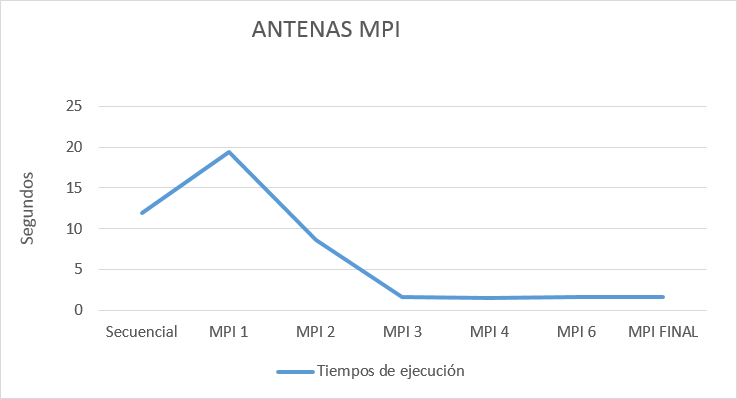
\includegraphics[width=0.8\textwidth]{./grafico.png}
\end{figure}

\end{document}
